%!TEX root = ../../_main.tex
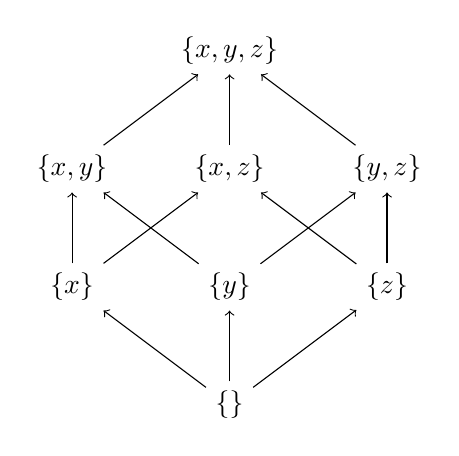
\begin{tikzpicture}
	\tikzstyle{every node}=[]
	\tikzstyle{relation}=[->]

	\node (xyz) at (0,0) {$\{x,y,z\}$};
	\node (xy) at (-2,-1.5) {$\{x,y\}$};
	\node (xz) at (0,-1.5) {$\{x,z\}$};
	\node (yz) at (2,-1.5) {$\{y,z\}$};
	\node (x) at (-2,-3) {$\{x\}$};
	\node (y) at (0,-3) {$\{y\}$};
	\node (z) at (2,-3) {$\{z\}$};
	\node (0) at (0,-4.5) {$\{\}$};
	\draw[relation] (0) -- (x);
	\draw[relation] (0) -- (y);
	\draw[relation] (0) -- (z);
	\draw[relation] (x) -- (xy);
	\draw[relation] (x) -- (xz);
	\draw[relation] (y) -- (xy);
	\draw[relation] (y) -- (yz);
	\draw[relation] (z) -- (xz);
	\draw[relation] (z) -- (yz);
	\draw[relation] (xy) -- (xyz);
	\draw[relation] (xz) -- (xyz);
	\draw[relation] (yz) -- (xyz);
\end{tikzpicture}